\documentclass[10pt,a4paper,landscape]{article}
\usepackage{multicol}
\usepackage{calc}
\usepackage{ifthen}
\usepackage[landscape]{geometry}
\usepackage{amsmath,amsthm,amsfonts,amssymb,mathtools}
\usepackage{color,graphicx}
\usepackage{hyperref}
\usepackage{listings}
\usepackage{underscore}
\usepackage{todonotes}

% Cheatsheet style
% Cheatsheet style

% This sets page margins to .5 inch if using letter paper, and to 1cm
% if using A4 paper. (This probably isn't strictly necessary.)
% If using another size paper, use default 1cm margins.
\ifthenelse{\lengthtest{\paperwidth = 11in}}
  % Then
  { \geometry{top=.5in,left=.5in,right=.5in,bottom=.5in} }
  % Else
  { \ifthenelse{\lengthtest{\paperwidth = 297mm}}
    {\geometry{top=1cm,left=1cm,right=1cm,bottom=1cm} }
    {\geometry{top=1cm,left=1cm,right=1cm,bottom=1cm} }
  }

% Turn off header and footer
\pagestyle{empty}

% Redefine section commands to use less space
\makeatletter
\renewcommand{\section}{\@startsection{section}{1}{0mm}%
                                {-1ex plus -.5ex minus -.2ex}%
                                {0.5ex plus .2ex}%x
                                {\color{darkred}\normalfont\large\bfseries}}
\renewcommand{\subsection}{\@startsection{subsection}{2}{0mm}%
                                {-1explus -.5ex minus -.2ex}%
                                {0.5ex plus .2ex}%
                                {\color{darkdarkred}\normalfont\normalsize\bfseries}}
\renewcommand{\subsubsection}{\@startsection{subsubsection}{3}{0mm}%
                                {-1ex plus -.5ex minus -.2ex}%
                                {1ex plus .2ex}%
                                {\normalfont\small\bfseries}}
\makeatother

% Define BibTeX command
\def\BibTeX{{\rm B\kern-.05em{\sc i\kern-.025em b}\kern-.08em
    T\kern-.1667em\lower.7ex\hbox{E}\kern-.125emX}}

% Don't print section numbers
\setcounter{secnumdepth}{0}

\setlength{\parindent}{0pt}
\setlength{\parskip}{0pt plus 0.5ex}

% Setting colors
\definecolor{lightgray}{rgb}{0.7,0.7,0.7}
\definecolor{lightergray}{rgb}{0.9,0.9,0.9}
\definecolor{darkblue}{rgb}{0.4,0.4,1}
\definecolor{darkred}{rgb}{0.9,0.2,0.2}
\definecolor{darkdarkred}{rgb}{0.6,0.0,0.0}
\definecolor{lightred}{rgb}{1,0.6,0.6}
\definecolor{lightgreen}{rgb}{0.6,1,0.6}
\definecolor{lightblue}{rgb}{0.6,0.8,1}
\definecolor{darkgreen}{rgb}{0.4,1,0.4}

% Set code listing style
\lstset {
    backgroundcolor=\color{lightgray},
    basicstyle=\ttfamily\scriptsize,
    breaklines=true,
}

\lstdefinestyle{bb}{
    backgroundcolor=\color{lightergray},
    frame=L,
    xleftmargin=\parindent,
}

% Set hyperlink style
\hypersetup{hidelinks}

% Enable figures
\newenvironment{colfig}
  {\par\medskip\noindent\minipage{\linewidth}}
  {\endminipage\par\medskip}

% Enable arg min/max math operators
\DeclareMathOperator*{\argmin}{arg\,min}
\DeclareMathOperator*{\argmax}{arg\,max}


% Shorthands
\providecommand{\bf}[1]{\ensuremath{\mathbf{#1}}}
\newcommand{\E}{\mathrm{E}}
\newcommand{\Var}{\mathrm{Var}}
\newcommand{\Cov}{\mathrm{Cov}}
\newcommand{\bbeta}{\boldsymbol\beta}
\newcommand{\bdelta}{\boldsymbol\delta}
\newcommand{\btheta}{\boldsymbol\theta}

\pdfinfo{
  /Title (Machine Learning Cheat Sheet)
  /Creator (TeX)
  /Producer (pdfTeX 1.40.0)
  /Author (Dennis Meier)
  /Subject (Machine Learning cheatsheet)
  /Keywords (machinelearning, ml, bayes, regression, classification)
}

% -----------------------------------------------------------------------

\begin{document}
\title{Machine Learning Cheat Sheet}

\raggedright
\footnotesize
\sffamily
\begin{multicols*}{4}

% multicol parameters
% These lengths are set only within the two main columns
%\setlength{\columnseprule}{0.25pt}
\setlength{\premulticols}{1pt}
\setlength{\postmulticols}{1pt}
\setlength{\multicolsep}{1pt}
\setlength{\columnsep}{2pt}

\begin{center}
\Large{\underline{Machine Learning Cheat Sheet}}
\end{center}

% ----------
\section{General}
\subsection{Dataset and Definitions}
$\mathcal{D}$ is a set of training examples, the n-th Training Example ($n = 1,2, ..., N$), of this set is: $\bf{x}_n = \begin{bmatrix} x_{n1} \quad x_{n2} \quad ... \quad x_{nD} \end{bmatrix}$

We write all N training examples in a matrix: $\bf{X} = \begin{bmatrix} \bf{x}_1 ; \quad \bf{x}_2 ; \quad ... ; \quad \bf{x}_N \end{bmatrix}$

In supervised learning, you are also given a set of observations corresponding to the training examples:  $\bf{y} = \begin{bmatrix} y_1 \quad y_2 \quad ... \quad y_{N} \end{bmatrix}^T$

We assume a \emph{true} model behind the data, the observations are noisy versions of this ground truth: $y = y_{true} + \epsilon$.

The final goal is to predict a $\hat{y} = f(\bf{\hat{x}})$ given any $\bf{\hat{x}}$.

\subsection{Distributions}
Multivariate gaussian distribution: $\mathcal{N}(\bf{X} | \bf{\mu} , \bf{\Sigma})$ \\
$\implies p(\bf{X} = \bf{x}) = (2 \pi)^{-d/2} |\bf{\Sigma|}^{-1/2} \exp{[- \frac{1}{2} (\bf{x} - \bf{\mu})^T \bf{\Sigma}^{-1} (\bf{x} - \bf{\mu})]}$

Gaussian distribution: $\mathcal{N}(X| \mu, \sigma^2)$ \\
$\implies p(X = x) = \frac{1}{\sqrt{2 \pi \sigma^2}} \exp{(- \frac{1}{2} ( \frac{x - \mu}{\sigma} )^2)}$

Poisson distribution: $\mathcal{P}(X| \lambda)$ \\
$\implies p(X = k) = \frac{\lambda ^ k}{k!} \exp{(- \lambda)}$

\subsection{Properties}
\textbf{Bayes rule}: $p(A, B) = p(A|B) p(B) = p(B|A) p(A)$

A matrix $\bf{M}$ is \textbf{positive semidefinite} $\iff \forall$ nonzero vector $\bf{a}$, we have $\bf{a}^T \bf{M} \bf{a} \geq 0$

\textbf{Jensen's inequality} applied to $\log$: $\log( \mathbb{E}[X] ) \geq \mathbb{E}[\log(X)]$ \\
$\implies \log ( \sum_x x \cdot p(x) ) \geq \sum_x p(x) \log(x)$

\textbf{Matrix inversion lemma}: $(\bf{PQ} + \bf{I}_N)^{-1} \bf{P} = \bf{P}(\bf{QP} + \bf{I}_M)^{-1}$

Useful derivative: $\frac{\partial \bf{x^T B x}}{\partial \bf{x}} = (\bf{B + B^T}) \bf{x}$

Marginal and Conditional Gaussians:
$$
\begin{aligned}
p(\bf{x}) &= \mathcal{N}(\bf{x} | \boldsymbol\mu, \boldsymbol\Lambda^-1) \\
p(\bf{y}|\bf{x}) &= \mathcal{N}(\bf{y} | \bf{Ax + b, L}^-1) \\
\Downarrow \\
p(\bf{y}) &= \mathcal{N}(\bf{y} | \bf{A} \boldsymbol\mu + \bf{b}, \bf{L}^-1 + \bf{A} \boldsymbol\Lambda^-1 \bf{A}^T)	\\
p(\bf{x}|\bf{y}) &= \mathcal{N}(\bf{x} |\boldsymbol\Sigma \{ \bf{L(y - b) + \Lambda \mu} \}, \boldsymbol\Sigma) \\
\text{where } \boldsymbol\Sigma &= (\boldsymbol\Lambda + \bf{A^T L A})^{-1}
\end{aligned}
$$

% ----------
\section{Optimization methods}

\subsection{Grid Search}
Simply try values for all parameters at regular intervals.
Complexity: $\mathcal{O}(M^D N D)$, where $M$ is the number of values tried in each dimension.

\subsection{Gradient Descent}
Update rule: $\bbeta^{(k+1)} = \bbeta^{(k)} - \alpha \frac{\partial \mathcal{L}(\bbeta^{(k)})}{\partial \bbeta}$

Complexity: $\mathcal{O}(I N D)$ where $I$ is the number of iterations we take.

$\alpha$ is a parameter that needs to be chosen carefully.

The gradient for MSE comes out as:
$\frac{\partial \mathcal{L}}{\partial \bbeta} = - \frac{1}{N} \tilde{X}^T ( \boldsymbol y - \tilde{X} \bbeta )$

\subsection{Newton's method}
It uses second order derivatives information to converge faster (we approximate the objective function by a quadratic function rather than a line).

General rule: $\bbeta^{(k+1)} = \bbeta^{(k)} - \alpha \bf{H_k^{-1}} \frac{\partial \mathcal{L}(\bbeta^{(k)})}{\partial \bbeta}$\\
where $\bf{H_k}$ is the $D \times D$ Hessian at step $k$: $\bf{H_k} = \frac{\partial^2 \mathcal{L}(\bbeta^{(k)})}{\partial \bbeta^2}$

Newton's method is equivalent to solving many least-squares problems.

Complexity: $\mathcal{O}(I N D^2 + I D^3)$, with the $D^3$ cost coming from the inversion of $\bf{H_k}$.

\subsection{Expectation-Maximization}
EM is a family of methods to find a MLE/MAP estimator if some of the data is missing (e.g. latent variables):

Given is some data $\bf{x}$ and  a model with some latent variables $\bf{z}$ and a likelihood $\mathcal{L}(\btheta; \bf{x}, \bf{z})$ (e.g. a gaussian where we need to find the mean and the covariance).
Goal is to find $\beta = \argmax_{\beta} \mathcal{L}_{lik}(\btheta; x)$, i.e. the MLE given only the data, without knowing the latent variables.

The problem is, that this likelihood can oftentimes not be optimized in closed form with respect to $\btheta$.

The solution is EM: Iteratively find better $\btheta$, start with $\btheta_0$ and iterate with variable $t$:
\begin{itemize}
\item E-step calculates the $\mathbb{E}$ of log likelihood, with respect to $\bf{Z}$ given $\bf{X}$ under the current estimate $\btheta_t$: $Q(\btheta, \btheta_t) = \mathbb{E}_{\bf{Z}|\bf{X},\btheta_t} [ log ( p(\bf{X}, \bf{Z} | \btheta) | X = x ]$
\item M-step finds next estimate that maximizes: $\btheta_{t+1} = \argmax_{\btheta} Q(\btheta, \btheta_t)$
\item Iterate until convergence.
\end{itemize}

% ----------
\section{Regression}
Simple linear regression: $y_n \approx \beta_0 + \beta_1 x_{n1}$

Multiple linear regression: $y_n \approx f(\bf{x}_n) := \beta_0 + \beta_1 x_{n1} + \beta_2 x_{n2} + ... + \beta_D x_{nD}$

\subsection{Linear basis function model}
We can create more complex models while staying in the linear framework by transforming the inputs $X$ of dimensionality $D$ through a function $\phi : D \rightarrow M$.

$y_n = \beta_0 + \sum_{i=1}^{M} \beta_i \phi_i(\bf{x_n}) =  \bf{\tilde\phi^T}(\bf{x}^T_n) \bbeta$.
The optimal $\beta$ can be computed in closed form by $\beta = ( \tilde{\Phi}^T \tilde{\Phi})^{-1} \tilde{\Phi}^T y$ where $\tilde{\Phi}$ is a matrix with N rows and the n-th row is $[1, \phi_1(x_n)^T,  ...,  \phi_M(x_n)^T]$. But note this requires $\tilde{\Phi}^T \tilde{\Phi}$ to be invertible (well-conditionned: $\tilde\phi$ full column-rank).

Ridge regression: $\beta_{ridge} = ( \tilde{\boldsymbol\Phi}^T \tilde{\boldsymbol\Phi} + \lambda \boldsymbol I)^{-1} \tilde{\boldsymbol\Phi}^T \boldsymbol y$

\subsection{Cost functions}
%\begin{colfig}
%\centering
%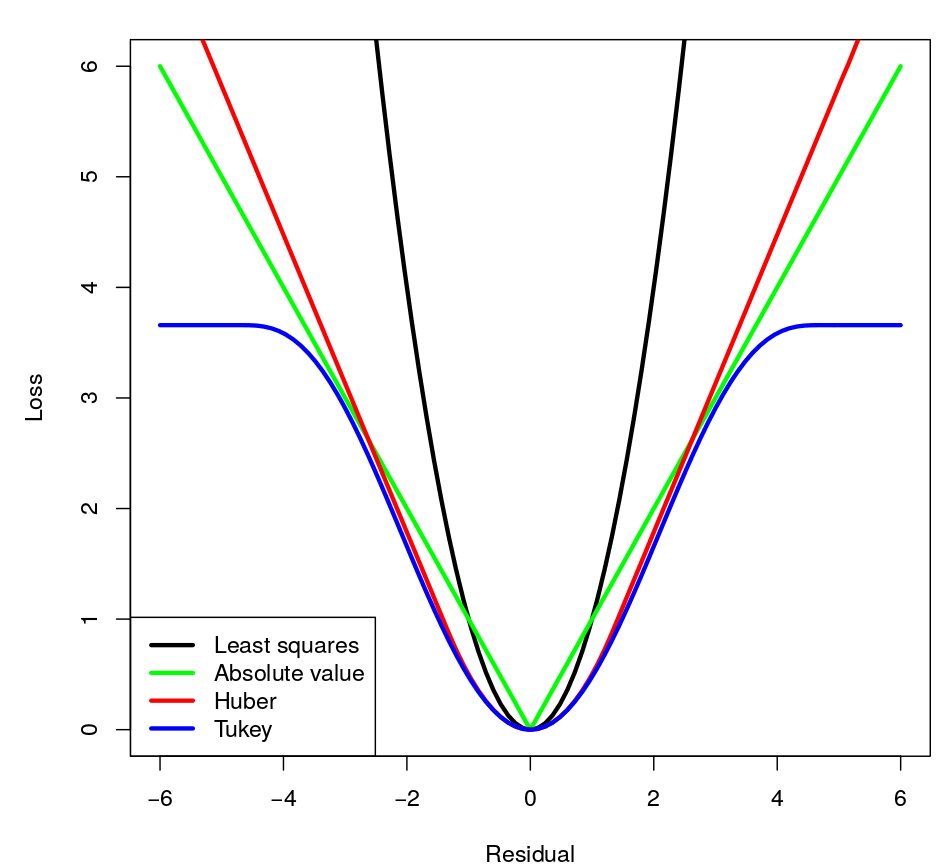
\includegraphics[width=\linewidth]{images/error-functions.png}
%\end{colfig}

Cost function / Loss: $\mathcal{L}(\bbeta) = \mathcal{L}(\mathcal{D},\bbeta)$

Mean square error (MSE): $\frac{1}{2N} \sum_{n=1}^{N}\left[y_n-f(\bf{x}_i) \right]^2$

MSE matrix formulation: $\frac{1}{2N} (\bf{y - X \beta})^T (\bf{y - X \beta})$

Mean absolute error (MAE): $\frac{1}{2N} \sum_{n=1}^{N}\left | y_n-f(\bf{x}_i) \right |$

Huber loss: $\mathcal{L}_\delta (a) = \begin{cases}
\frac{1}{2}{a^2}                   & \text{for } |a| \le \delta, \\
\delta (|a| - \frac{1}{2}\delta ), & \text{otherwise.}
\end{cases}$

Root mean square error (RMSE): $\sqrt{2 * \text{MSE}}$

Epsilon insensitive (``hinge loss'', used for SVM):
$\mathcal{L}_{\epsilon}(y, \hat{y}) = \begin{cases}
0                   & \text{if } |y - \hat y| \le \epsilon, \\
|y - \hat y| - \epsilon, & \text{otherwise.}
\end{cases}$

% ----------
\section{Least squares}
Complexity: $\mathcal{O}(ND^2 + D^3)$
The gradient of the MSE set to zero is called the normal equation:
$$ - \bf{y^T X} + \bf{X^T X \bbeta} = 0$$
We can solve this for $\beta$ directly (by matrix manipulation)
$\bbeta = ( \bf{\tilde{X}}^T \bf{\tilde{X}} )^{-1} \bf{\tilde{X}}^T y$

% ----------
\section{Classification}
Logistic Function: $\sigma(t) = \frac{exp(t)}{1+exp(t)}$\\
Derivative: $\frac{ \partial\sigma(t) }{ \partial t } = \sigma(t)[ 1 - \sigma(t) ]$

Classification with linear regression: Use $y = 0$ as class $\mathcal{C}_1$
and $y = 1$ as class $\mathcal{C}_2$ and then decide a newly estimated $y$ belongs
to $\mathcal{C}_1$ if $y < 0.5$.

\subsection{Logistic Regression}
$\frac{ \partial\mathcal{L}(\bbeta) }{ \partial \bbeta } = \tilde{\bf{X}}^T [\sigma(\tilde{\bf{X}} \beta) - \bf{y}]$

There's no closed form, we can use gradient descent.

\subsection{Generalized linear model}
The GLM consists of three elements:
\begin{itemize}
  \item A probability distribution from the exponential family.
  \item A linear predictor $\hat y = \bf{X} \bf{\beta}$ .
  \item A link function g such that $E(y) = \mu = g^{-1}(\eta)$.
\end{itemize}

In a generalized linear model (GLM), each outcome of the dependent variables $y$ is assumed to be generated from a particular distribution in the exponential family, a large range of probability distributions that includes the normal, binomial, Poisson and gamma distributions, among others.


\subsection{Cost functions}
RMSE: $\sqrt{\frac{1}{N} \sum_{n=1}^{N}\left[y_n- \hat{p_n} \right]^2}$

0-1 Loss: $ \frac{1}{N} \sum_{n=1}^{N} \delta(y_n, \hat{y_n})$

Log-Loss: $- \frac{1}{N}  \sum_{n=1}^{N} y_n \log(\hat{p_n}) + (1-y_n) \log(1-\hat{p_n})$

% ----------
\section{Probabilistic framework}
The Likelihood Function maps the model parameters to the probability distribution of $\bf{y}$:
$\mathcal{L}_{lik}\colon \text{parameter space} \to [0;1]\quad  \bf{\beta} \mapsto p(\bf{y} \mid  \bf{\beta})$
An underlying $p$ is assumed before. If the observed $y$ are IID, $p(\bf{y} \mid \beta) = \prod_n p(y_n \mid \beta)$.

$\mathcal{L}_{lik}$ can be viewed as just another cost function. Maximum likelihood then simply chooses the parameters $\bf{\beta}$ such that observed data is most likely. $\beta = \argmax_{\text{all} \beta} L(\beta)$

Assuming different $p$ is basically what makes this so flexible. We can chose e.g.:

\begin{tabular}{ l  l }
  \hline
  Gaussian $p$ & $\mathcal{L}_{lik} \widehat{=} -\mathcal{L}_{MSE}$ \\
  Poisson $p$  & $\mathcal{L}_{lik} \widehat{=} -\mathcal{L}_{MAE}$ \\
  \hline
\end{tabular}

It is a sample approximation of the expected likelihood:
$\mathcal{L}_{lik}(\boldsymbol{\beta}) \approx E_y[ p(y \mid  \boldsymbol{\beta}) ]$

\subsection{Bayesian methods}
Bayes rule: $p(A, B) = p(A|B) p(B) = p(B|A) p(A)$

The \textbf{prior} $p(\bf{f}|\bf{X})$ encodes our prior belief about the ``true'' model $\bf{f}$. The \textbf{likelihood} $p(\bf{y}|\bf{f})$ measures the probability of our (possibly noisy) observations given the prior.

Least-squares tries to find model parameters $\bf{\beta}$ which maximize the likelihood. Ridge regression maximizes the \textbf{posterior} $p(\bf{\beta}|\bf{y})$

\subsection{Bayesian networks}
We can use a Directed Acyclic Graph (DAG) to define a joint distribution of events. For example, we can express the relationship between \textit{latent factors} (possible ``causes'') $z_i$ and \textit{observations} (results) $y_i$:

\begin{colfig}
  \centering
  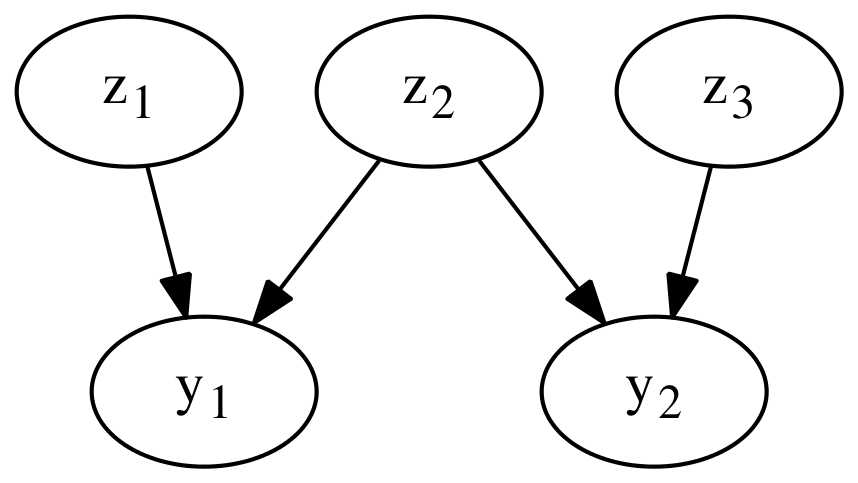
\includegraphics[height=1.5cm]{images/bayesian-network.png}
\end{colfig}

This example can be factorized as follows:
$p(y_1, y_2, z_1, z_2, z_3) = p(y_1 | z_1, z_2) p(y_2 | z_2, z_3) p(z_1) p(z_2) p(z_3)$

We can then obtain the distribution over latent factors ($z_i$) by marginalizing over the unknown variables:
$p(z_1, z_2, z_3 | y_1, y_2) = \frac{\text{joint}}{p(y_1, y_2)}$\\
$\implies p(z_1 | y_1, y_2) = \sum_{z_2, z_3} \frac{\text{joint}}{p(y_1, y_2)}$

\subsection{Belief propagation}
Belief propagation is a message-passing based algorithm used to compute desired marginals (e.g. $p(z_1 | y_1, y_2)$) efficiently. It leverages the factorized expression of the joint. Messages passed:

$m_{z_i \rightarrow y_j} = p(z_i) \Pi(\text{messages received except from } y_j)$

$m_{y_j \rightarrow z_i} = \sum_{z_k \neq z_i} p(y_j | z_k) \Pi(\text{messages received except from } z_i)$

% ----------
\section{Kernel methods}
Kernels are another way to encode our prior believe about the relation of outputs to inputs. A kernel defines a distance measure, or ``similarity'' of two vectors. We define:

$(\bf{K})_{i,j} = \kappa(\bf{x_i}, \bf{x_j}) = \vec \phi(\bf{x_i})^T \vec \phi(\bf{x_j})$.

The $\phi$ are not that important in the end, because we only use the Kernel as is. Sometimes it's even impossible to write them down explicitly.

\begin{tabular}{ l | l }
  \hline
  Linear     & $\kappa(\bf{x_i}, \bf{x_j}) = \bf{x_i}^T \bf{x_j}$ \\
  \hline
  Polynomial & $\kappa(\bf{x_i}, \bf{x_j}) = (\bf{x_i}^T \bf{x_j} + c)^d$ \\
  \hline
  RBF        & $\kappa(\bf{x_i}, \bf{x_j}) = \exp\left(-\frac{||\bf{x_i} - \bf{x_j}||^2}{2\sigma^2}\right)$ \\
  \hline
\end{tabular}

Properties of a Kernel:
\begin{itemize}
\item $\bf{K}$ should be symmetric: $\bf{K}^T = \bf{K}$
\item $\bf{K}$ should be positive semi-definite: $\forall$ nonzero vector $\bf{a}, \bf{a}^T \bf{K} \bf{a} \geq 0$.
\end{itemize}

\subsection{Gaussian Process}
The predicting function $f$ is interpreted as a random variable with jointly gaussian prior: $\mathcal{N}(f | \bf{0}, \bf{K})$.
Defining the Kernel matrix $\bf{K} = \kappa(\bf{X}, \bf{X})$ defines the prior. The key idea is, that if $\bf{x}_i$ and $\bf{x_j}$ are
deemed by the kernel to be similar, then we expect the output of $f$ at those points to be similar, too.

We can sample functions from this random variable $f$ and we can use prior + measurements to generate predictions.

If we have measurements $\bf{y}$ available, we get a joint distribution with the $\bf{\hat{y}}$ to be predicted:

$
\begin{bmatrix}
  \bf{y} \\
  \bf{\hat{y}}
\end{bmatrix}
=
\mathcal{N} \left(
  \bf{0},
  \begin{bmatrix}
    \kappa(\bf{X}, \bf{X}) + \sigma_n^2 I  & \kappa(\bf{X}, \bf{\hat{X}}) \\
    \kappa(\bf{\hat{X}}, \bf{X}),          & \kappa(\bf{\hat{X}}, \bf{\hat{X}})
  \end{bmatrix}
\right)
$

This can be conditioned on $\bf{y}$ to find the PDF of $\bf{\hat{y}}$. Advantage: we output our prediction as probabilities (which represent uncertainty).

% ----------
\section{Neural Networks}
A feed forward Neural Network is organized in $K$ layers, each layer with $M^{(k)}$ hidden units $z_i^{(k)}$. Activations $a_i^{(k)}$ are computed as the linear combination of the previous layer's terms, with weights $\bbeta^{(k)}$ (one $M^{(k-1)} \times 1$ vector of weights for each of the $M^{(k)}$ activations). Activations are then passed through a (possibly nonlinear) function $h$ to compute the hidden unit $z_i^{(k)}$.

$\bf{x}_n \xrightarrow{\bbeta_i^{(1)}} a_i^{(1)} \xrightarrow{h} z_i^{(1)} \xrightarrow{\bbeta^{(2)}} \dots \bf{z}^{(K)} = \bf{y}_n$

\subsection{Backpropagation}
It's an algorithm which computes the gradient of the cost $\mathcal{L}$ w.r.t. the parameters $\bbeta^{(k)}$.

Forward pass: compute $a_i$, $z_i$ and $\bf{y}_n$ from $\bf{x}_n$.

Backward pass: work out derivatives from outputs to the target $\bbeta_i^{(k)}$. Using the chain rule:\\
$\bdelta^{(k-1)} = \frac{\partial \mathcal{L}}{\partial \bf{a}^{(k-1)}} = diag[ h'(\bf{a}^{(k-1)}) ] \bf{B^{(k)T}} \bdelta^{(k)}$\\
$\frac{\partial \mathcal{L}}{\partial \bf{B}^{(1)}} = \bdelta^{(1)} \bf{x}^T$\\
$\frac{\partial \mathcal{L}}{\partial \bf{B}^{(k)}} = \bdelta^{(k)} \bf{z}^{(k)T}$

\subsection{Regularization}
NN are not \textit{identifiable} (existence of many local optima), therefore the maximum likelihood estimator is not \textit{consistent}.

NN are universal density estimators, and thus prone to severe overfitting. Techniques used to reduce overfitting include early stopping (stop optimizing when test error starts increasing) and ``weight decay'' (i.e. $L_2$ regularization).

% ----------
\section{Support Vector Machines}
Search for the hyperplane separating the data such that the gap (margin) is biggest.
It minimizes the following cost function (``hinge loss''):

$\mathcal{L}_{SVM} (\bf{\beta})= \sum_{n=1}^N [1 - y_n \tilde\phi_n \beta]_{+} + \frac{\lambda}{2} \sum_{j=1}^M \beta_j^2$

with $[t]_{+} = \max(0, t)$

This is convex but not differentiable. In the dual, the same problem can be formulated as:

$\max_{\alpha \in [0; C]^N} \alpha^T 1 - 1/2 \alpha^T Y K Y \alpha , \alpha^T y = 0$

% ----------
\section{Gaussian Mixture Models}
In mixture models, the data is generated by a sum (a mix) of $K$ models. For GMM, these are gaussian:

$p(\bf{x}_i | \theta) = \sum_{k=1}^K \pi_k p_k(\bf{x}_i | \theta) =  \sum_{k=1}^K \pi_k \mathcal{N}(\bf{x}_i | \underbrace{\bf{\mu}_k, \bf{\Sigma}_k}_{\theta})$

To use this for clustering, we first fit this mixture and then compute the posterior $p(z_i = k | \bf{x}_i, \theta)$. This yields \textit{soft} cluster assignments.

% ----------
\section{PCA}
Find the eigenvectors of the covariance matrix $\bf{X^T X}$ of the data. These form an orthonormal basis $\{ \bf{w}_1, ..., \bf{w}_N\}$ for the data in the directions that have highest variance.
One can then use the first $L < D$ vectors to rebuild the data: $\bf{\hat{x}}_i = \bf{W} \bf{z}_i = \bf{W} \bf{W}^T \bf{x}_i$, with $\bf{W} = \begin{bmatrix} \bf{w}_1 ; ... ; \bf{w}_L \end{bmatrix}$.
This minimizes mean square error $\frac{1}{N} \sum_{i=1}^N \bf{x}_i - \bf{\hat{x}}_i^2$.

\section{SVD}
The same as with PCA, we can do with SVD:
\begin{colfig}
  \centering
  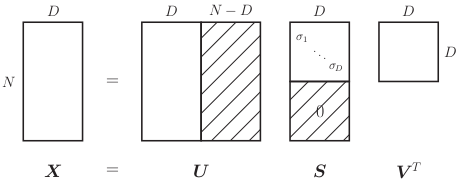
\includegraphics[width=\linewidth]{images/svd.png}
\end{colfig}

The singular vals of a $N \times D$ matrix $\bf{X}$ are the square roots of the eigenvalues of the $D \times D$ matrix $\bf{X^T X}$
% ----------
\section{Concepts}

\subsection{Convexity}
f is called convex f: $\forall x_1, x_2 \in X, \forall t \in [0, 1]: \qquad f(tx_1+(1-t)x_2)\leq t f(x_1)+(1-t)f(x_2).$

Sum of two convex functions is convex. Composition of a convex function with a convex, nondecreasing function is convex. Linear, exponential and $\log(\sum \exp)$ functions are convex.

\subsection{Bias-Variance Decomposition}
\begin{colfig}
  \centering
  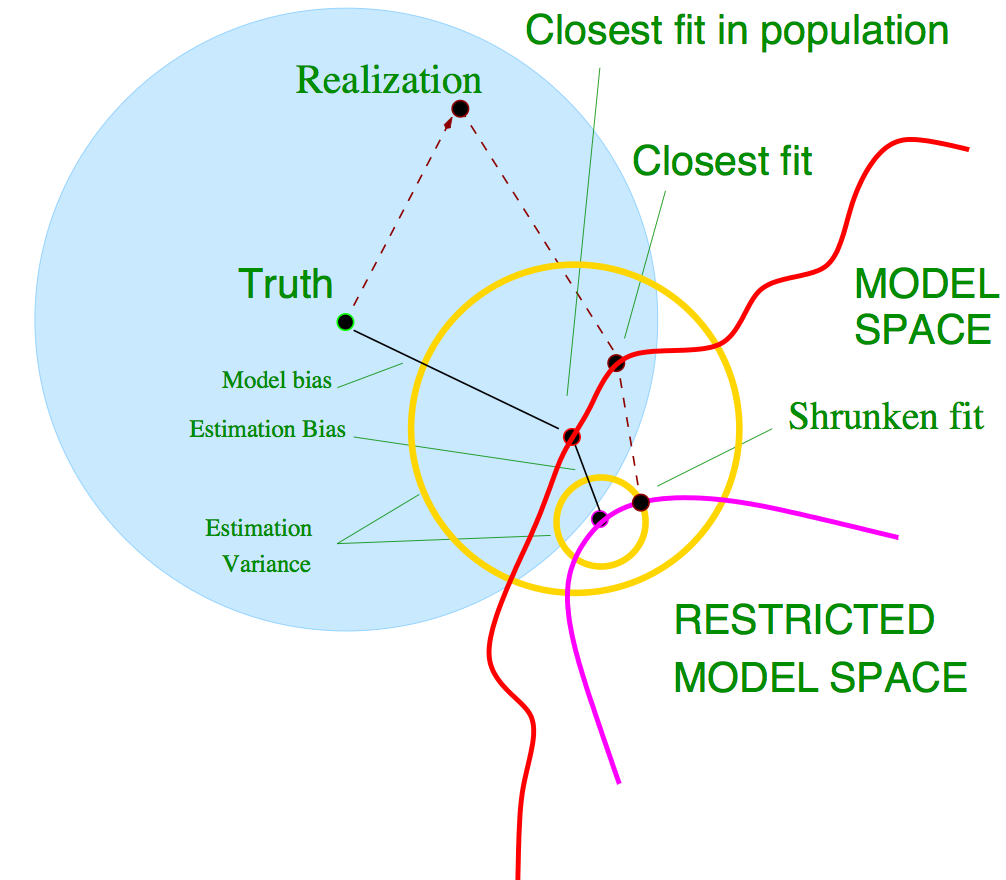
\includegraphics[width=\linewidth]{images/bias-variance.png}
\end{colfig}

Bias-variance comes directly out of the test error:
 \begin{align*}
 \overline{teErr}
 &= E[(\text{observation} - \text{prediction})^2] = E[(y - \hat{y})^2] \\
 &= E[(y - y_{true} + y_{true} - \hat{y})^2] \\
 &=\underbrace{E[(y - y_{true})^2]}_{\text{var of measurement}} + E[(y_{true} - \hat{y})^2] \\
 &=\sigma^2 + E[(y_{true} - E[\hat{y}] + E[\hat{y}] - \hat{y})^2] \\
 &=\sigma^2 + \underbrace{E[(y_{true} - E[\hat{y}])^2]}_{\text{pred bias}^2} +\underbrace{E[(E[\hat{y}] - \hat{y})^2]}_{\text{pred variance}}
\end{align*}

\begin{tabular}{ l || c | c }
                          & bias & variance \\
  \hline
  regularization          & +    & - \\
  choose simpler model    & +    & - \\
  more data               & -    & \\
  \hline
\end{tabular}

\subsection{Identifiability}
We say that a statistical model $\mathcal{P} = \{P_\theta: \theta \in \Theta\}$ is identifiable if the mapping $\theta \mapsto P_\theta$ is one-to-one:
$P_{\theta_1}=P_{\theta_2} \quad\Rightarrow\quad \theta_1=\theta_2 \quad\ \text{for all } \theta_1,\theta_2\in\Theta.$

A non-identifiable model will typically have many local optima yielding the same cost, e.g. $\mathcal{L}(W, Z) = \mathcal{L}(aW, \frac{1}{a} Z)$

\subsection{Curse of dimensionality}
With the dimensionality increase, every data point becomes arbitrarily far
from every other data point and therefore the choice of nearest neighbor becomes random.
In high dimension, data only covers a tiny fraction of the input space, making generalization extremely difficult.
Or in other words, the volume of the space increases so fast that the available data become sparse.

\subsection{Primal vs. Dual}
Instead of working in the \textbf{column space} of our data, we can work in the \textbf{row space}:
$$\bf{\hat{y} = X \beta = X X^T \alpha = K \alpha}$$
where $\bf{\beta} \in \mathbb{R}^D$ and $\bf{\alpha} \in \mathbb{R}^N$
and (like magic) $\bf{K}$ shows up, the Kernel Matrix.

Representer Theorem: For any $\bf{\beta}$ minimizing
$$\min_\beta \sum_{n=1}^N \mathcal{L}(y_n, \bf{x}_n^T \bf{\beta}) + \sum_{d=1}^D \lambda \beta_d^2$$
there exists an $\bf{\alpha}$ such that $\bf{\beta = X^T \alpha}$.

When we have an explicit vector formulation of $\beta$, we can use the matrix inversion lemma to get to the dual. E.g. for ridge regression:
$$\beta = (X^T X  + \lambda I_D)^{-1} X^T y = X^T \underbrace{(X X^T + \lambda I_N)^{-1} y}_{\alpha}$$

In optimization, we get to the dual like this:
\begin{colfig}
  \centering
  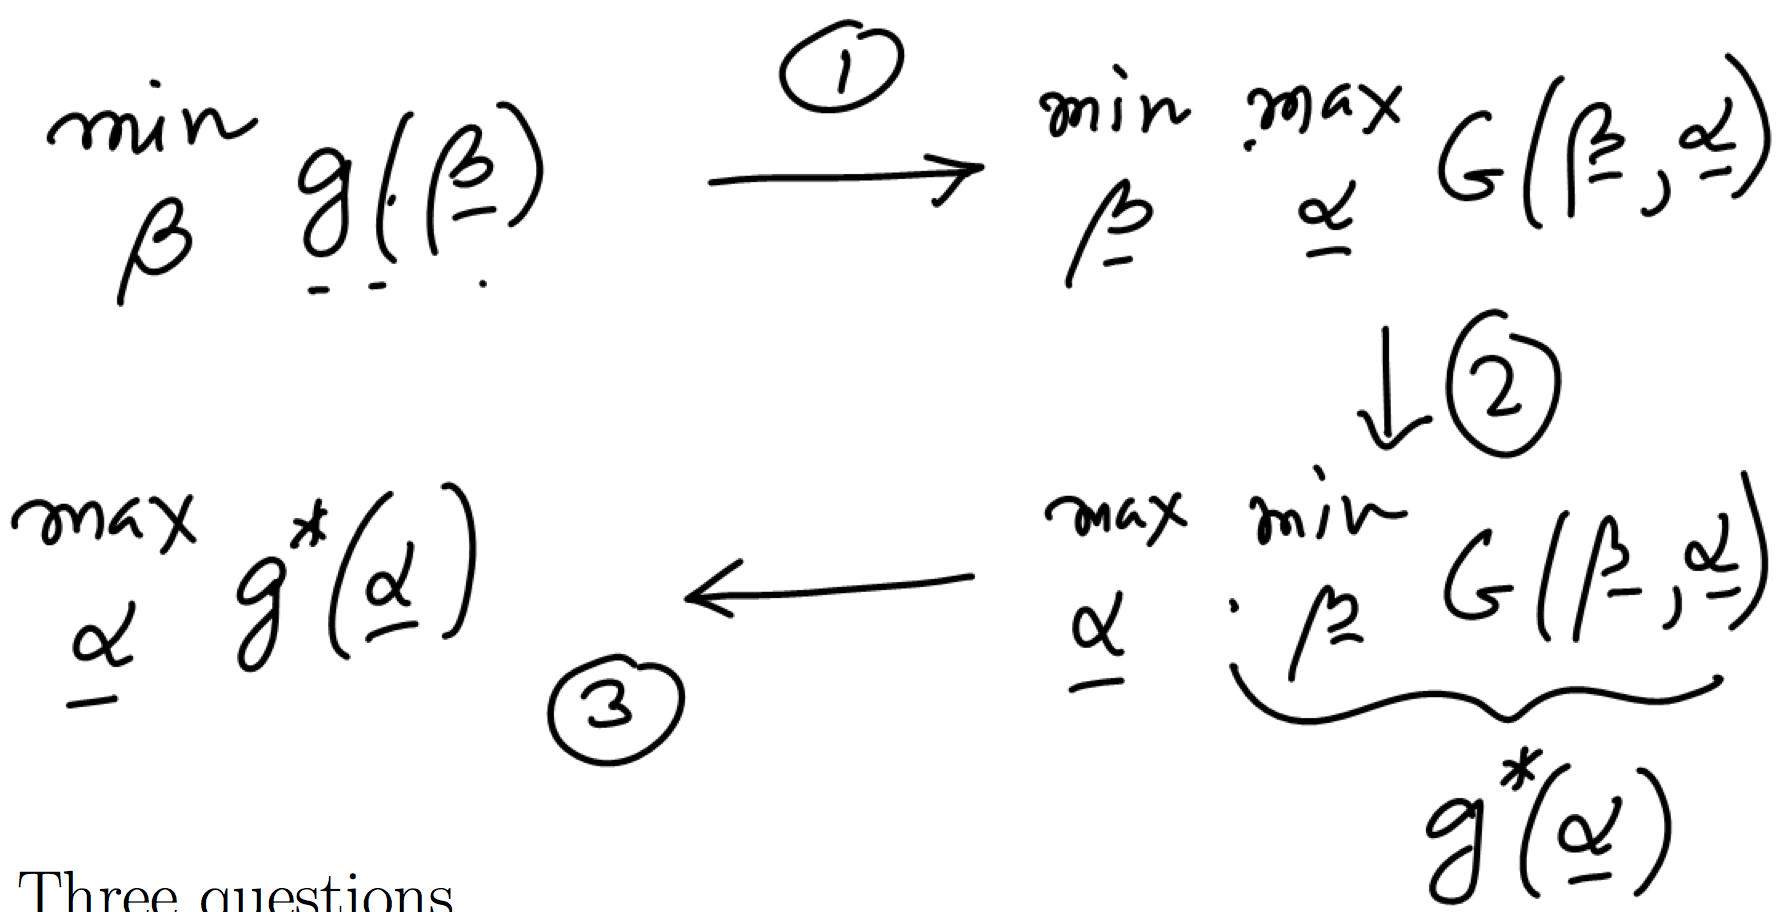
\includegraphics[width=\linewidth]{images/prim-dual.png}
\end{colfig}

% ----- Less useful concepts
\subsection{Consistency}
An estimator is said to be consistent, if it eventually recovers the true parameters that generated the data as the sample size goes to infinity. Of course, this only makes sense if the data actually comes from the specified model, which is not usually the case. Nevertheless, it can be a useful theoretical property.

\subsection{Efficiency}
An estimator is called efficient if it achives the Cramer-Rao lower bound:
$\Var{(\beta)} \geq 1/I(\beta)$, where I is the Fisher information.

\subsection{Occam's Razor}
It states that among competing hypotheses, the one with the fewest assumptions should be selected. Other, more complicated solutions may ultimately prove correct, but in the absence of certainty, the fewer assumptions that are made, the better.

\todo[inline]{TODO: K-fold cross-validation, definition of Test-Error, Train-Error}

\todo[inline]{TODO: statistical goodness (robust to outliers, ...) vs. computational goodness (convex, low computational complexity, ...) tradeoff. No free lunch theorem.}

\todo[inline]{TODO: Decision Trees and Random Forests and Model averaging}

% ---------- Credits
\section{Credits}
Most material was taken from the lecture notes of \href{http://people.epfl.ch/228491}{Prof. Emtiyaz Khan}.\\
Cost functions figure from Patrick Breheny's slides.\\
Biais-variance decomposition figure from Hastie, Tibshirani, Friedman, \textit{The Elements of Statistical Learning}.
The SVD figure from Kevin P. Murphy, \textit{Machine Learning, A Probabilistic Perspective}.

% ---------- Footer
\hrule
\tiny
Rendered \today. Written by Dennis Meier and Merlin Nimier-David.
\copyright Dennis Meier. This work is licensed under the Creative Commons Attribution-ShareAlike 3.0 Unported License.
To view a copy of this license, visit \href{http://creativecommons.org/licenses/by-sa/3.0/}{http://creativecommons.org/licenses/by-sa/3.0/} or
send a letter to Creative Commons, 444 Castro Street, Suite 900, Mountain View, California, 94041, USA.

\includegraphics{images/by-sa.png}

\end{multicols*}
\end{document}
